% ============================================================================
% Presentación oral — Trabajo Práctico Final de Deep Learning  (VERSIÓN 2)
% Sistema de Detección y Segmentación de Objetos en Tiempo Real
% Autor: Federico Morán
% Compilar: pdflatex presentacion2.tex  (dos pasadas)
%
% Cambios respecto de presentacion.tex (v1, 34 láminas):
%   - Se eliminan TODAS las láminas de código (antiguas 7, 8 y el listado de la
%     demo en tiempo real) y el paquete `listings`.
%   - Se fusionan láminas afines para bajar de 29 a 17 láminas de exposición
%     (objetivo: 10 minutos).
%   - Las curvas de aprendizaje pasan a los anexos.
%   - NARRATIVA: la comparación SESGADA contra el baseline (sobre nuestro test de
%     train2017) sale del cuerpo principal y queda como lámina de respaldo. En el
%     cuerpo se presenta únicamente la comparación IMPARCIAL sobre val2017,
%     explicando cómo se construyó.
%   - La ablación (ajuste completo vs. backbone congelado) sube de los anexos a la
%     lámina de resultados: es donde valida la decisión de congelar, anunciada en
%     la lámina del modelo.
%   - Se conservan todas las figuras narrativas.
% ============================================================================
\documentclass[aspectratio=169,11pt]{beamer}

\usepackage[utf8]{inputenc}
\usepackage[T1]{fontenc}
\usepackage{lmodern}
\usepackage[spanish,es-tabla,es-noquoting]{babel}
\usepackage{graphicx}
\usepackage{booktabs}
\usepackage{amsmath}
\usepackage{xcolor}
\usepackage{tikz}
\usetikzlibrary{arrows.meta,positioning,shapes.geometric}

\usetheme{Boadilla}
\setbeamertemplate{navigation symbols}{}
\setbeamertemplate{caption}[numbered]
\setbeamercovered{transparent}

% --- Paleta coherente con las figuras del informe -----------------------------
\definecolor{azul}{HTML}{2A78D6}
\definecolor{aqua}{HTML}{1BAF7A}
\definecolor{ambar}{HTML}{EDA100}
\definecolor{rojo}{HTML}{E34948}
\definecolor{gris}{HTML}{5A5A5A}

\setbeamercolor{structure}{fg=azul}
\setbeamercolor{title}{fg=white,bg=azul}
\setbeamercolor{frametitle}{fg=white,bg=azul}
\setbeamercolor{block title}{fg=white,bg=azul}
\setbeamercolor{block title alerted}{fg=white,bg=rojo}
\setbeamercolor{block title example}{fg=white,bg=aqua}
\setbeamerfont{frametitle}{size=\large}
\setbeamerfont{title}{series=\bfseries}

\graphicspath{{../reporte/figuras/}}

% Pie de página compacto
\setbeamertemplate{footline}{%
  \hbox{%
    \begin{beamercolorbox}[wd=.5\paperwidth,ht=2.4ex,dp=1ex,leftskip=1em]{author in head/foot}%
      \usebeamerfont{author in head/foot}\insertshortauthor
    \end{beamercolorbox}%
    \begin{beamercolorbox}[wd=.5\paperwidth,ht=2.4ex,dp=1ex,rightskip=1em]{author in head/foot}%
      \hfill\insertframenumber{} / \inserttotalframenumber
    \end{beamercolorbox}}%
  \vskip0pt%
}

\title[Detección y segmentación en tiempo real]{Sistema de Detección y Segmentación de
Objetos en Tiempo Real mediante Ajuste Fino de YOLOv8}
\subtitle{Trabajo Práctico Final --- Deep Learning}
\author[Federico Morán]{Federico Morán}
\institute[Maestría en IA]{Maestría en Inteligencia Artificial}
\date{Julio de 2026}

\begin{document}

% ============================================================================
\begin{frame}[plain]
  \titlepage
\end{frame}

% ============================================================================
\begin{frame}{Contenidos}
  \begin{columns}[T]
    \begin{column}{0.52\textwidth}
      \tableofcontents
    \end{column}
    \begin{column}{0.44\textwidth}
      \begin{block}{Hilo conductor}
        \footnotesize
        Ajustar un modelo de segmentación de instancias y llevarlo a tiempo real
        sobre una CPU\ldots \textbf{y descubrir que medir bien el resultado es tan
        difícil como obtenerlo.}
      \end{block}
    \end{column}
  \end{columns}
\end{frame}

% ============================================================================
\section{Problema y alcance}

\begin{frame}{Problema, objetivo y alcance}
  \begin{columns}[T]
    \begin{column}{0.52\textwidth}
      \begin{block}{Objetivo}
        \footnotesize
        Un sistema completo de visión por computadora que \textbf{detecte y segmente
        objetos en tiempo real} sobre hardware de consumo: datos $\rightarrow$ ajuste
        fino $\rightarrow$ evaluación $\rightarrow$ inferencia en vivo.
        \vspace{0.3em}

        \textbf{¿Por qué el tiempo real?} Robótica, asistencia y análisis de video exigen
        \textbf{precisión} y \textbf{latencia} a la vez, sobre todo sin aceleración
        dedicada.
      \end{block}
      \vspace{0.2em}

      \textbf{Ocho clases}\\[0.2em]
      {\small\texttt{person} \enskip \texttt{cell phone} \enskip \texttt{cup} \enskip
      \texttt{bottle}\\
      \texttt{laptop} \enskip \texttt{keyboard} \enskip \texttt{mouse} \enskip
      \texttt{book}}
      \vspace{0.25em}

      {\scriptsize \textbf{Criterio:} todas pueden \textbf{exhibirse físicamente} ante una
      cámara web en la demo: es un criterio de aplicación, no de conveniencia estadística.
      Las 72 categorías restantes de COCO pasan a ser \textbf{fondo}, lo que define con
      precisión el alcance del problema.}
    \end{column}
    \begin{column}{0.46\textwidth}
      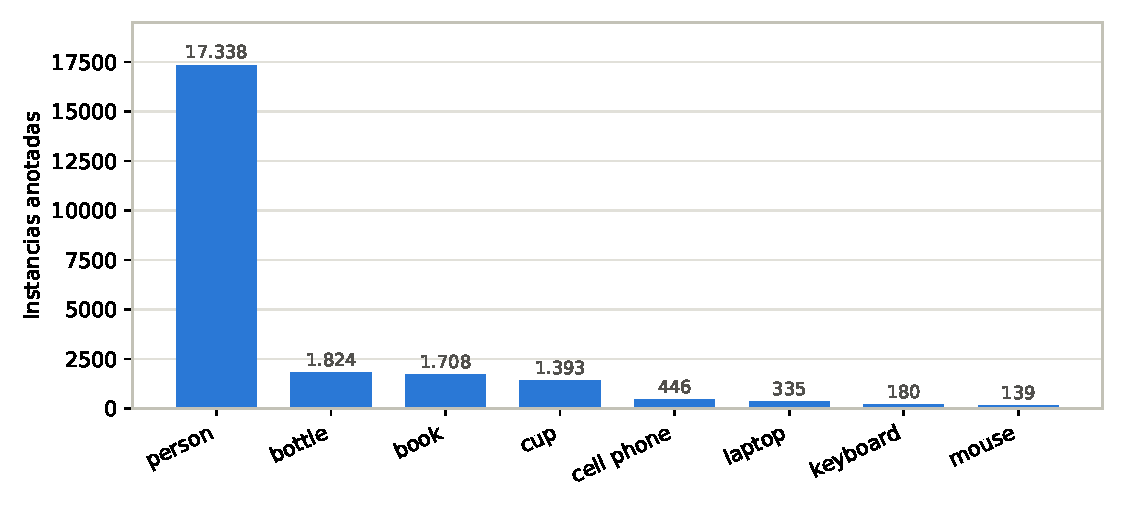
\includegraphics[width=\textwidth]{dist_clases.pdf}
      \\[0.3em]
      {\scriptsize Desbalance pronunciado, heredado de la estadística natural de COCO:
      \texttt{person} concentra el 74,2\,\% de las instancias; \texttt{mouse} reúne 139.}
    \end{column}
  \end{columns}
\end{frame}

\begin{frame}{Dos tareas, un modelo --- y las anotaciones que lo permiten}
  \begin{columns}[T]
    \begin{column}{0.48\textwidth}
      \textbf{Detección} --- localiza cada objeto con una \emph{caja delimitadora} y le
      asigna una clase.
      \vspace{0.5em}

      \textbf{Segmentación de instancias} --- delimita, \emph{píxel a píxel}, la silueta
      exacta de cada objeto individual.
      \vspace{0.6em}

      \begin{exampleblock}{Clave}
        \footnotesize
        YOLOv8-seg resuelve \textbf{ambas} tareas en una única pasada hacia adelante: la
        cabeza predice caja, clase y coeficientes de máscara simultáneamente.
      \end{exampleblock}
      \vspace{0.4em}

      {\footnotesize Por eso el conjunto de datos se anota a nivel de \textbf{instancia}
      (polígonos, no solo cajas): 5.000 imágenes y 23.363 instancias de COCO 2017.}
    \end{column}
    \begin{column}{0.48\textwidth}
      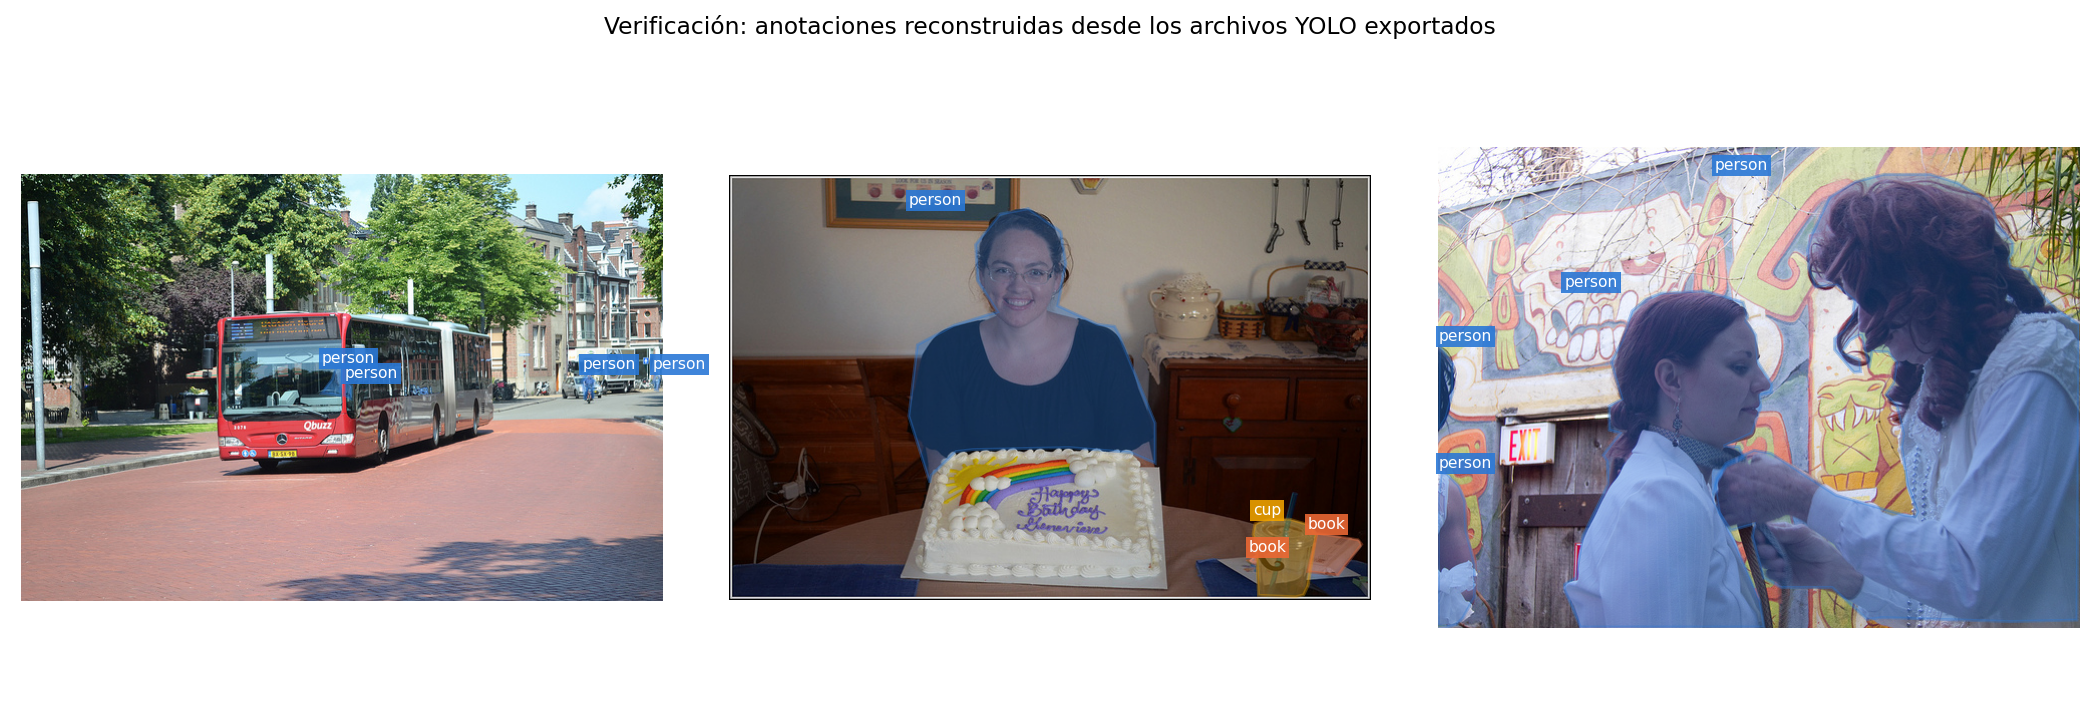
\includegraphics[width=\textwidth]{verificacion_etiquetas.png}
      \\[0.3em]
      {\scriptsize \textbf{Control de calidad:} las anotaciones se reconstruyen \emph{desde
      los archivos YOLO exportados} y se superponen sobre las imágenes. Valida la cadena
      completa: formato, normalización de coordenadas y asignación de índices de clase.}
    \end{column}
  \end{columns}
\end{frame}

% ============================================================================
\section{Datos, modelo y entrenamiento}

\begin{frame}{Pipeline de extremo a extremo}
  \centering
  \scalebox{0.92}{%
  \begin{tikzpicture}[
      node distance=0.38cm and 0.45cm,
      caja/.style={rectangle, rounded corners=2pt, draw=azul!70, fill=azul!8,
                   text width=2.3cm, align=center, font=\scriptsize, minimum height=1.1cm},
      cajav/.style={caja, draw=aqua!80, fill=aqua!10},
      flecha/.style={-{Stealth[length=2mm]}, draw=gris, thick}]

    \node[caja] (a) {Descarga selectiva\\COCO 2017\\{\tiny (FiftyOne, semilla fija)}};
    \node[caja, right=of a] (b) {Filtrado a\\las 8 clases};
    \node[caja, right=of b] (c) {Particiones\\60 / 15 / 25\,\%};
    \node[caja, right=of c] (d) {Export formato\\YOLO-seg\\{\tiny + saneamiento}};
    \node[cajav, below=0.9cm of d] (e) {Ajuste fino\\YOLOv8n-seg\\{\tiny GPU RTX 5090}};
    \node[cajav, left=of e] (f) {Evaluación\\mAP / IoU\\{\tiny partición de prueba}};
    \node[cajav, left=of f] (g) {Exportación\\OpenVINO};
    \node[cajav, left=of g] (h) {Inferencia en\\tiempo real\\{\tiny webcam + nube}};

    \draw[flecha] (a) -- (b);
    \draw[flecha] (b) -- (c);
    \draw[flecha] (c) -- (d);
    \draw[flecha] (d) -- (e);
    \draw[flecha] (e) -- (f);
    \draw[flecha] (f) -- (g);
    \draw[flecha] (g) -- (h);
  \end{tikzpicture}}

  \vspace{0.7em}
  \begin{columns}[T]
    \begin{column}{0.47\textwidth}
      \begin{block}{Particiones disjuntas a nivel de imagen}
        \footnotesize
        \textbf{3.000} entrenamiento \enskip / \enskip \textbf{750} validación \enskip /
        \enskip \textbf{1.250} prueba.\\
        La prueba queda reservada: no interviene en ninguna decisión.
      \end{block}
    \end{column}
    \begin{column}{0.47\textwidth}
      \begin{exampleblock}{Reproducibilidad y controles}
        \footnotesize
        Semillas fijas en todo el pipeline. Un \textbf{control de integridad sobre los
        archivos exportados} ---lo que el entrenador realmente lee--- verifica que las
        particiones sean disjuntas y detiene la corrida si no lo son.
      \end{exampleblock}
    \end{column}
  \end{columns}
\end{frame}

\begin{frame}{Modelo y estrategia: por qué congelamos el backbone}
  \begin{itemize}\footnotesize
    \item \textbf{YOLOv8n-seg} --- una etapa, libre de anclas: \emph{backbone} CSPDarknet
          $\rightarrow$ \emph{neck} PAN-FPN $\rightarrow$ cabeza desacoplada (caja, clase y
          \emph{coeficientes de máscara}) $+$ rama de \emph{prototipos}.
          \\{\scriptsize La máscara es una combinación lineal de prototipos
          $\Rightarrow$ costo de segmentación casi constante por imagen.}
    \item \textbf{Variante \emph{nano}} (3,26~M de parámetros) --- el tiempo real debe darse
          \textbf{sobre CPU}, sin GPU dedicada.
    \item \textbf{Se parte de los pesos preentrenados en COCO}, pero el vocabulario baja de
          80 a 8 clases:
      \begin{itemize}\scriptsize
        \item[\textcolor{aqua}{$\blacktriangleright$}] \textcolor{aqua}{\textbf{Se hereda}}
              --- backbone y neck completos: las representaciones visuales aprendidas sobre
              118.000 imágenes.
        \item[\textcolor{rojo}{$\blacktriangleright$}]
              \textcolor{rojo}{\textbf{Se reinicializa}} --- 36 tensores
              ($\sim$372.000 parámetros): \textbf{toda la rama de clasificación de la
              cabeza}, cuyas dimensiones dependen de \texttt{nc}.
      \end{itemize}
    \item El propio entrenador lo declara:
          {\ttfamily\scriptsize\color{gris}Overriding nc=80 with nc=8\quad
          \color{rojo}Transferred 381/417 items}
  \end{itemize}

  \vspace{0.3em}
  \begin{alertblock}{Decisión: congelar el backbone (\texttt{freeze=10})}
    \footnotesize
    El clasificador arranca \textbf{desde cero} y solo hay 3.000 imágenes: 40$\times$ menos
    que el preentrenamiento. Reentrenar la red entera arriesga \textbf{destruir
    representaciones buenas} para reaprenderlas con muy pocos datos $\Rightarrow$ se congela
    el backbone y todo el presupuesto de optimización va al \emph{neck} y a la cabeza.
    \textbf{La ablación de la próxima sección confirma que era la decisión correcta.}
  \end{alertblock}
\end{frame}

\begin{frame}{Entrenamiento: aumento de datos y configuración}
  \begin{columns}[T]
    \begin{column}{0.56\textwidth}
      {\scriptsize
      \begin{tabular}{@{}llp{2.6cm}@{}}
        \toprule
        \textbf{Transformación} & \textbf{Valor} & \textbf{Justificación} \\
        \midrule
        \emph{Mosaic} & 1,0 & Contextos y escalas atípicos \\
        Volteo horizontal & $p{=}0{,}5$ & Sin quiralidad relevante \\
        Traslación & $\pm$10\,\% & Encuadres imperfectos \\
        Escala & $\pm$50\,\% & Distancia objeto--cámara \\
        HSV & $0{,}015 / 0{,}7 / 0{,}4$ & Iluminación y color \\
        \bottomrule
      \end{tabular}}

      \vspace{0.4em}
      {\scriptsize Transforma de manera consistente las imágenes \emph{y} sus polígonos.
      \emph{Mosaic} se desactiva en las últimas 10 épocas. \textbf{Se omiten} volteo
      vertical, rotaciones y \emph{mixup}: generarían poses inverosímiles para el dominio.
      Entrada $640\times640$ por \emph{letterbox}.}

      \vspace{0.5em}
      {\scriptsize
      \begin{tabular}{@{}ll@{}}
        \toprule
        Base / estrategia & \texttt{yolov8n-seg.pt}, \texttt{freeze=10} \\
        Épocas & 150 (early stop en la 140) \\
        Lote / optimizador & 32 / AdamW, $lr_0 = 8{,}33\times10^{-4}$ \\
        Hardware / duración & RTX 5090 --- 132 min \\
        \bottomrule
      \end{tabular}}
    \end{column}
    \begin{column}{0.42\textwidth}
      \centering
      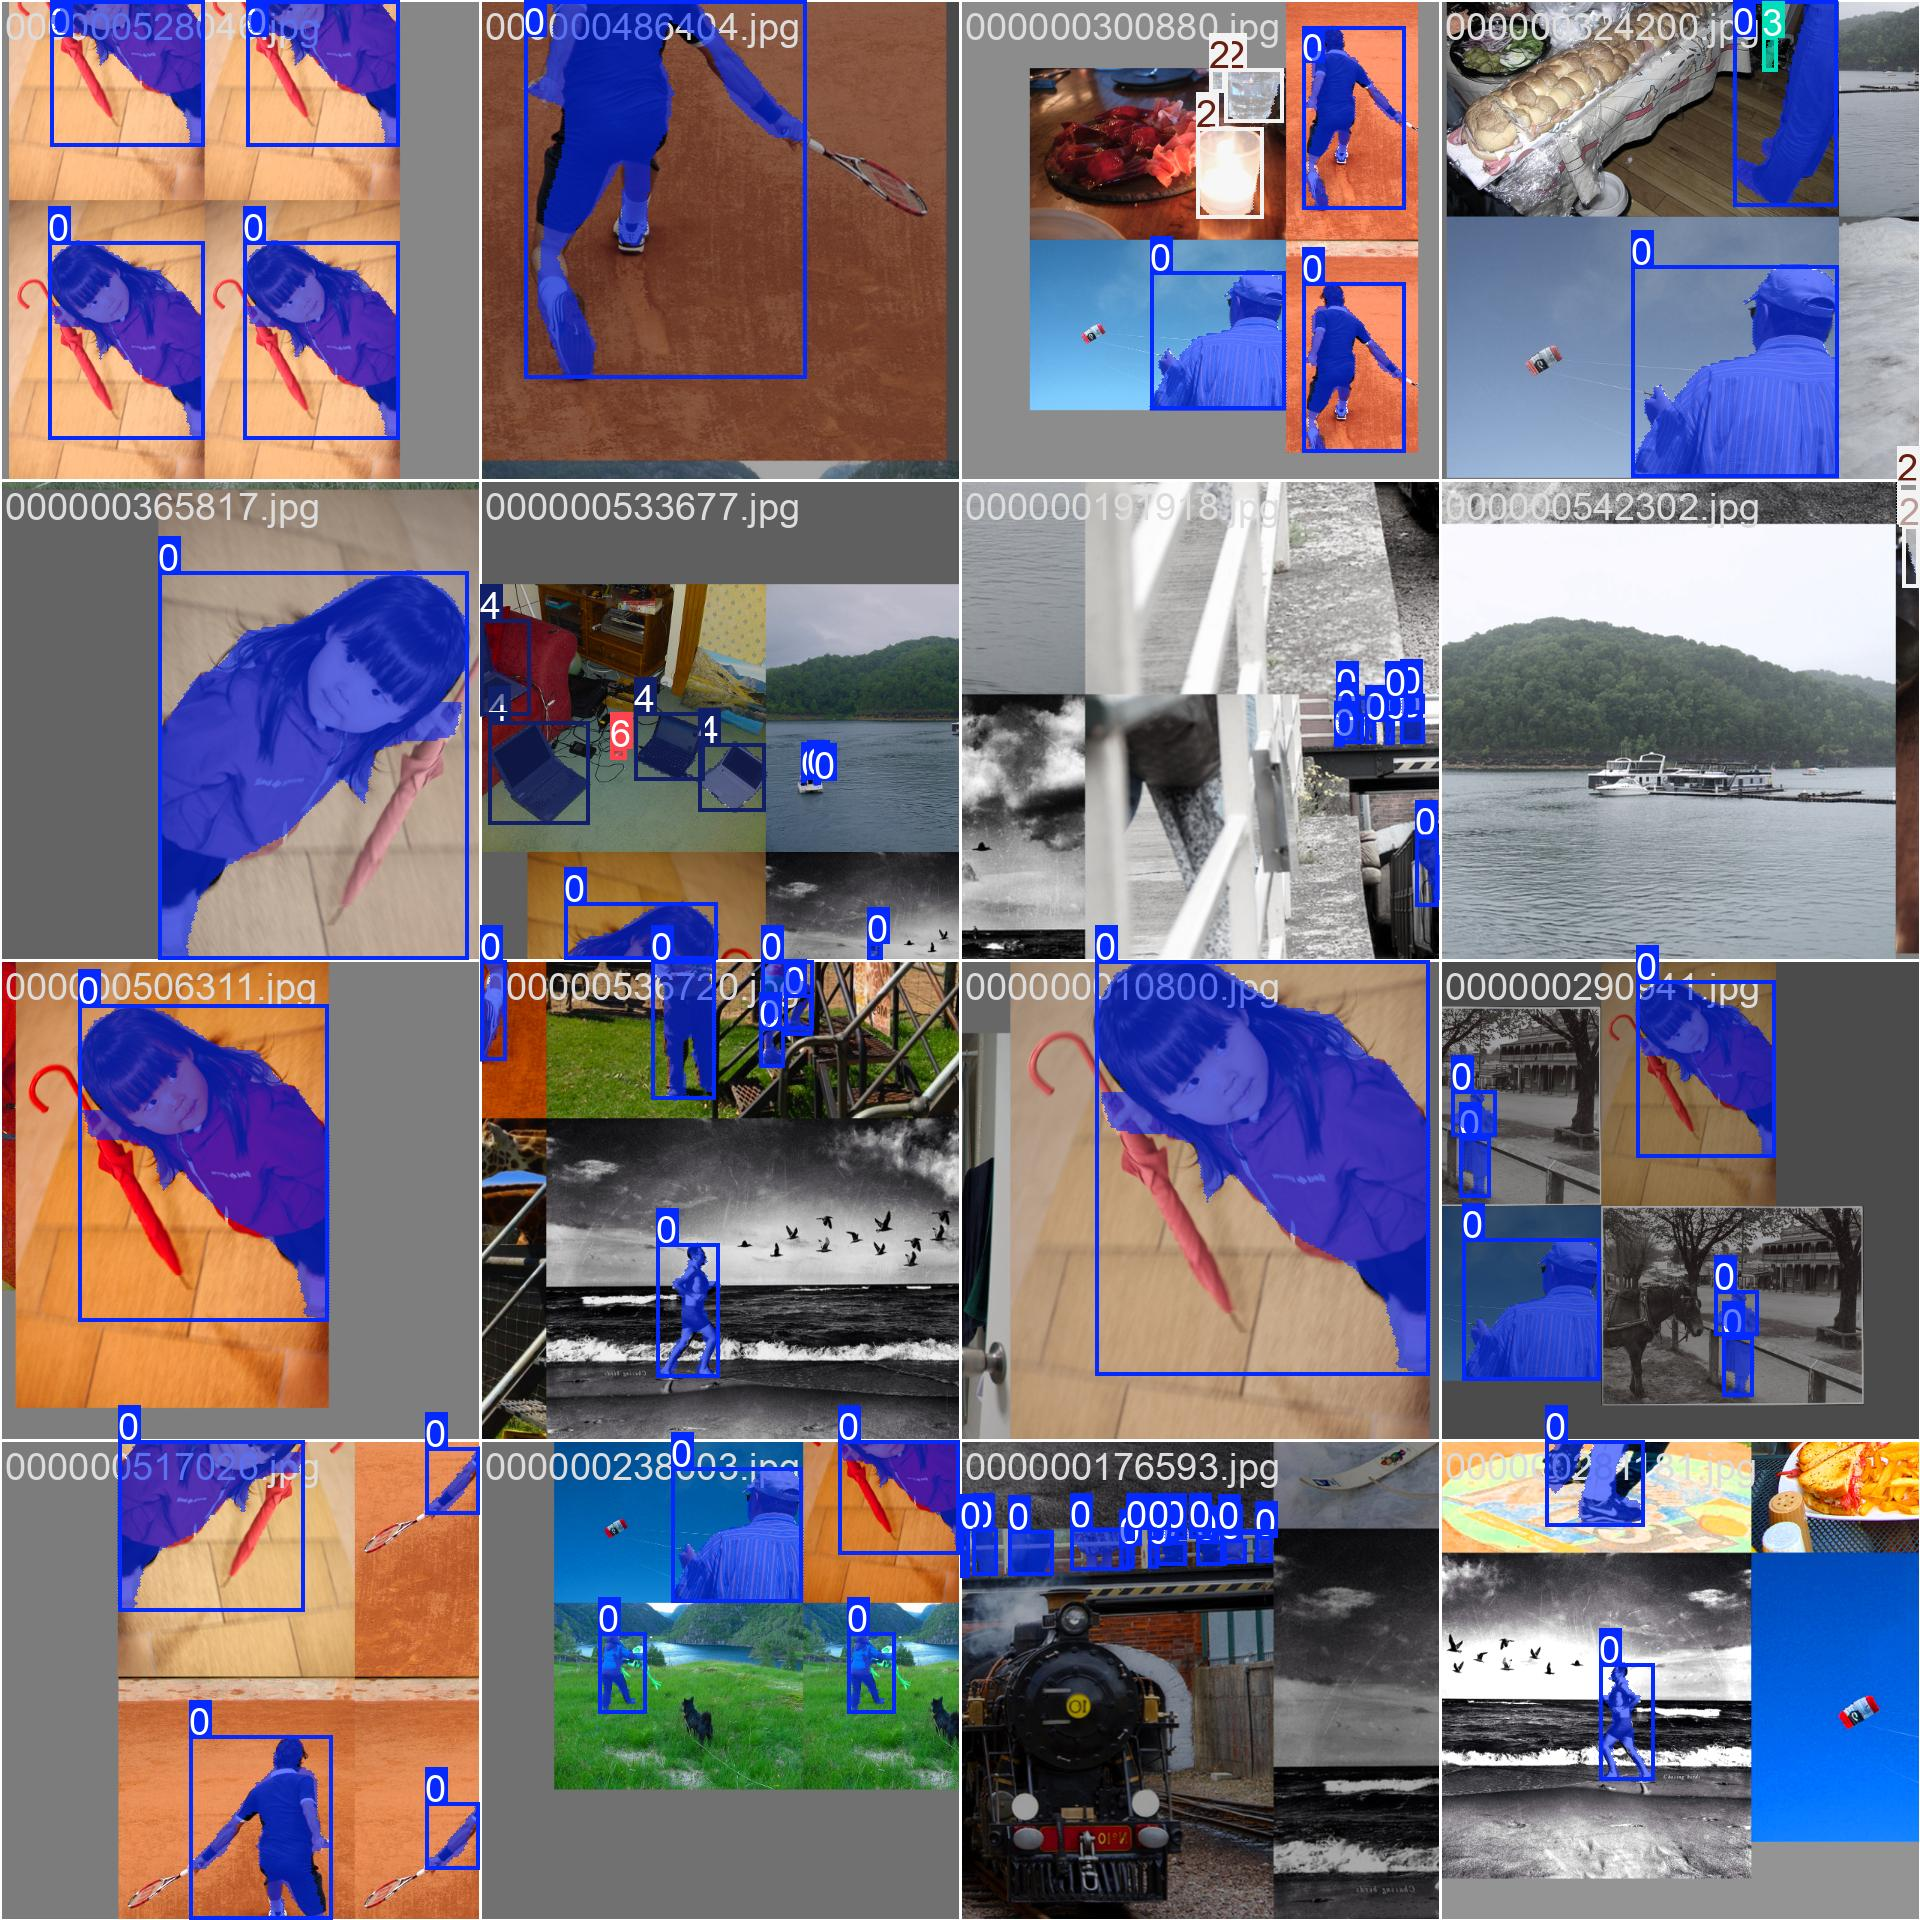
\includegraphics[width=0.80\textwidth]{mosaico_entrenamiento.jpg}
      \\[0.3em]
      {\scriptsize El punto de control se selecciona por la métrica de aptitud sobre
      \textbf{validación}. Curvas de aprendizaje en los anexos: sin sobreajuste.}
    \end{column}
  \end{columns}
\end{frame}

% ============================================================================
\section{Evaluación y resultados}

\begin{frame}{Resultados sobre la partición de prueba reservada}
  \begin{columns}[T]
    \begin{column}{0.53\textwidth}
      \centering
      {\small
      \begin{tabular}{@{}lcc@{}}
        \toprule
        \textbf{Modelo ajustado} & \textbf{Cajas} & \textbf{Máscaras} \\
        \midrule
        Precisión media & 0,577 & 0,559 \\
        Recall medio    & 0,397 & 0,383 \\
        mAP@50          & 0,440 & 0,420 \\
        mAP@50-95       & \textbf{0,292} & \textbf{0,246} \\
        \bottomrule
      \end{tabular}}

      \vspace{0.4em}
      \raggedright
      {\scriptsize \textbf{mAP@50-95} ---promedio sobre umbrales de IoU de 0,5 a 0,95--- es
      la métrica principal: premia la \textbf{precisión de la localización}. Se calcula por
      separado para cajas y máscaras sobre 1.250 imágenes y 7.117 instancias.}

      \vspace{0.4em}
      \begin{block}{El recall es el cuello de botella}
        \scriptsize
        La precisión (0,577) supera con holgura al recall (0,397): el modelo acierta cuando
        detecta, pero \textbf{omite} instancias. Las máscaras puntúan por debajo de las
        cajas: el IoU a nivel de píxel es más estricto.
      \end{block}
    \end{column}
    \begin{column}{0.45\textwidth}
      \begin{exampleblock}{Ablación: el congelamiento estaba justificado}
        \scriptsize
        \centering
        \begin{tabular}{@{}lcc@{}}
          \toprule
          \textbf{Configuración} & \textbf{Cajas} & \textbf{Másc.} \\
          \midrule
          Ajuste fino \emph{completo}, 60 ép. & 0,250 & 0,216 \\
          \textbf{Backbone congelado}, 150 ép. & \textbf{0,292} & \textbf{0,246} \\
          \bottomrule
        \end{tabular}

        \vspace{0.5em}
        \raggedright
        Ambas corridas parten de la \textbf{misma cabeza reinicializada}. Reentrenar la red
        entera con 3.000 imágenes \emph{degrada} el modelo: se pierden representaciones que
        COCO tardó 118.000 imágenes en construir.
      \end{exampleblock}
      \vspace{0.2em}
      {\scriptsize \textbf{Lección:} cuando el vocabulario de destino es un
      \textbf{subconjunto} del de preentrenamiento, un ajuste fino ingenuo puede
      \emph{empeorar} el modelo. Congelar el backbone vuelve \textbf{segura} la
      transferencia.}
    \end{column}
  \end{columns}
\end{frame}

\begin{frame}{¿Dónde falla el modelo?}
  \begin{columns}[T]
    \begin{column}{0.5\textwidth}
      \centering
      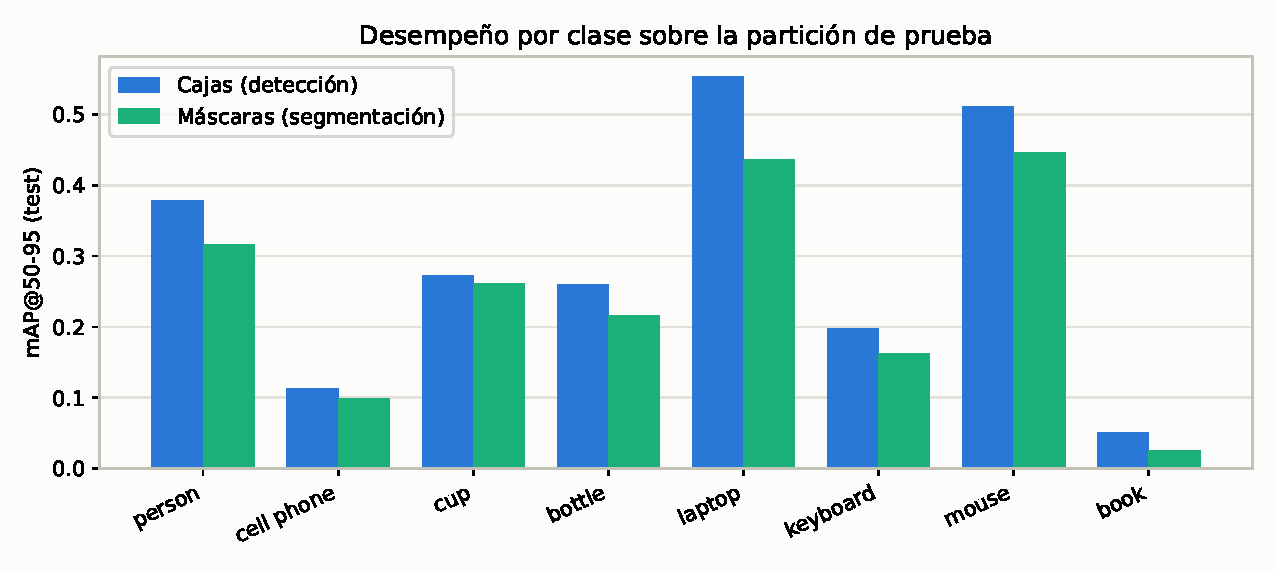
\includegraphics[width=0.95\textwidth]{map_por_clase.pdf}
      \\[0.1em]
      \raggedright
      {\scriptsize Mejores: \texttt{laptop} (0,554) y \texttt{mouse} (0,512), objetos
      rígidos y poco ocluidos. Peor: \texttt{book}, apilado en estanterías, con límites
      ambiguos y anotación inconsistente.}
    \end{column}
    \begin{column}{0.5\textwidth}
      \centering
      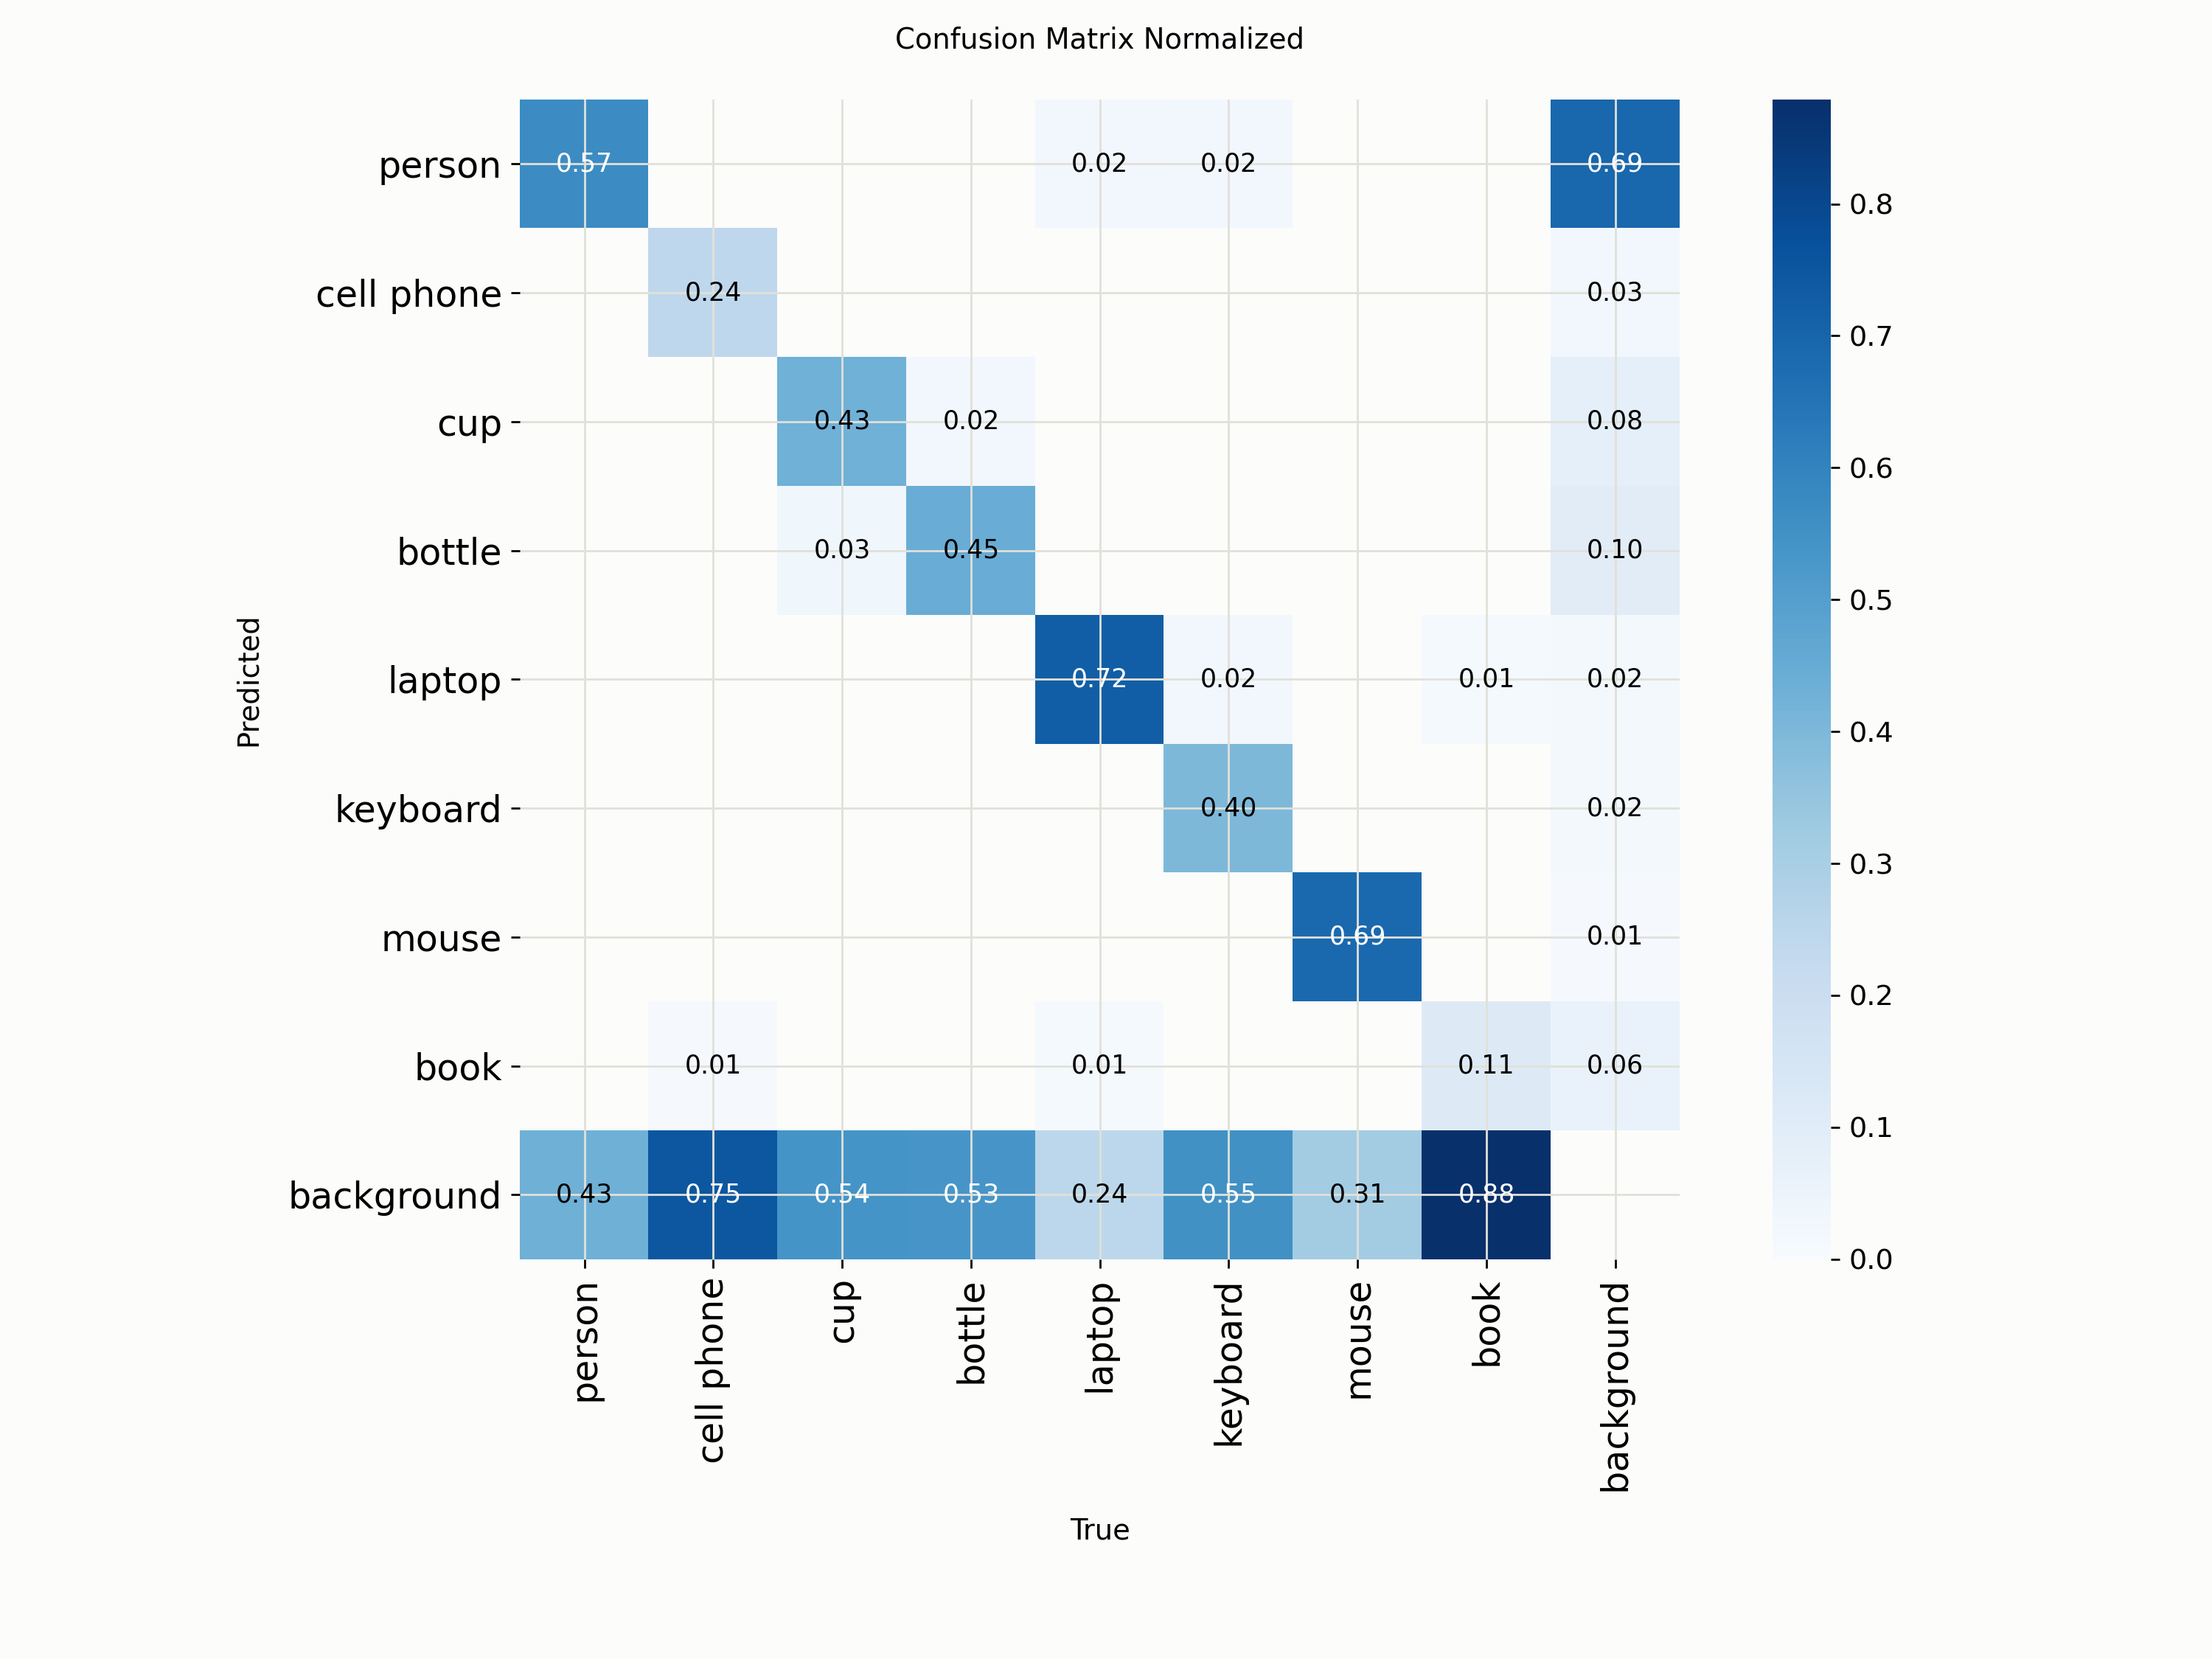
\includegraphics[width=0.62\textwidth]{confusion_matrix.png}
      \\[0.1em]
      \raggedright
      {\scriptsize El modelo \textbf{prácticamente no confunde clases entre sí}
      (máx.\ 0,03). El modo de error dominante es la \textbf{omisión}: objetos reales
      clasificados como fondo (\texttt{book} 88\,\%, \texttt{cell phone} 75\,\%).}
    \end{column}
  \end{columns}

  \vspace{0.4em}
  \begin{block}{Lectura conjunta}
    \footnotesize
    Con un vocabulario reducido la \emph{clasificación} es sencilla; lo difícil es
    \emph{detectar} instancias pequeñas u ocluidas. El margen de mejora está en el
    \textbf{recall}, no en la discriminación entre clases.
  \end{block}
\end{frame}

\begin{frame}{Comparación con el preentrenado: cómo hacerla bien}
  \begin{alertblock}{El problema: no se puede comparar sobre nuestra partición de prueba}
    \footnotesize
    El baseline (\texttt{yolov8n-seg.pt}) se entrenó sobre COCO~\textbf{train2017}, el mismo
    conjunto del que muestreamos nuestras 5.000 imágenes. \textbf{Ya vio, durante su
    preentrenamiento, las imágenes que nosotros usamos como prueba}, mientras que nuestro
    modelo se evalúa sobre datos genuinamente reservados. Medirlos ahí no compararía
    modelos: compararía memoria contra generalización.
  \end{alertblock}

  \vspace{0.5em}
  \begin{exampleblock}{La solución: un tercer conjunto que ninguno de los dos vio}
    \footnotesize
    Se replicó la receta de datos del Notebook~01 sobre \textbf{COCO val2017} ---el conjunto
    de validación oficial, \textbf{disjunto de train2017}, que el preentrenado nunca usó
    para ajustar sus pesos--- y se obtuvieron \textbf{1.250 imágenes nuevas}. Ambos modelos
    se evalúan sobre \emph{esas mismas} imágenes, cada uno con su vocabulario nativo (80 y 8
    clases); del baseline se extraen las AP de las 8 clases de interés.
    \vspace{0.3em}

    $\Rightarrow$ Ninguno de los dos vio los datos: \textbf{la comparación es limpia}.
  \end{exampleblock}
\end{frame}

\begin{frame}{Resultado de la comparación imparcial (COCO val2017)}
  \begin{columns}[T]
    \begin{column}{0.56\textwidth}
      \centering
      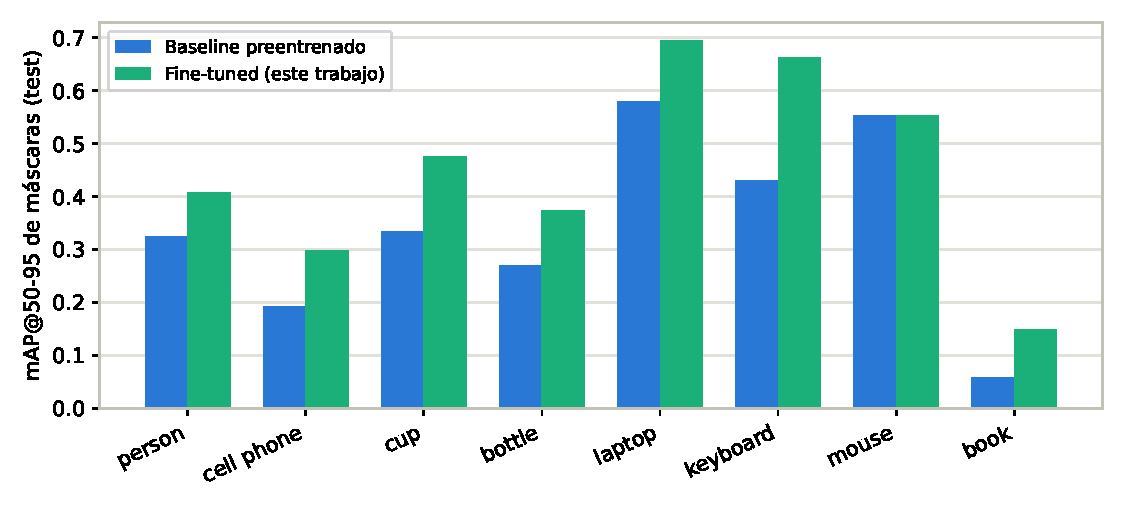
\includegraphics[width=\textwidth]{baseline_vs_finetuned.pdf}
    \end{column}
    \begin{column}{0.42\textwidth}
      \footnotesize
      \centering
      \begin{tabular}{@{}lcc@{}}
        \toprule
        mAP@50-95 & Preentr. & Ajustado \\
        \midrule
        Máscaras & 0,277 & 0,236 \\
        Cajas & 0,329 & 0,275 \\
        \bottomrule
      \end{tabular}
      \vspace{0.6em}

      \raggedright
      Sobre datos que ninguno vio, el modelo ajustado queda a \textbf{0,041} del
      preentrenado, con \textbf{paridad} en \texttt{person} ($-$0,008) y \texttt{mouse}
      ($-$0,007). La mayor diferencia persiste en \texttt{keyboard} ($-$0,115), la clase con
      menos ejemplos de entrenamiento (116).
    \end{column}
  \end{columns}

  \vspace{0.3em}
  \begin{block}{Por qué el preentrenado es un baseline tan fuerte --- y qué significa igualarlo}
    \footnotesize
    Las 8 clases son un \textbf{subconjunto} de su vocabulario: las aprendió sobre 118.000
    imágenes. Ajustar con 3.000 del mismo dominio no agrega información nueva, así que lo
    esperable es \textbf{igualarlo, no superarlo en mAP}. Entonces, ¿para qué sirvió el
    ajuste fino?
  \end{block}
\end{frame}

\begin{frame}{Entonces, ¿qué aporta el ajuste fino? Especialización}
  \begin{columns}[T]
    \begin{column}{0.5\textwidth}
      \centering {\scriptsize Baseline (80 clases)}\\
      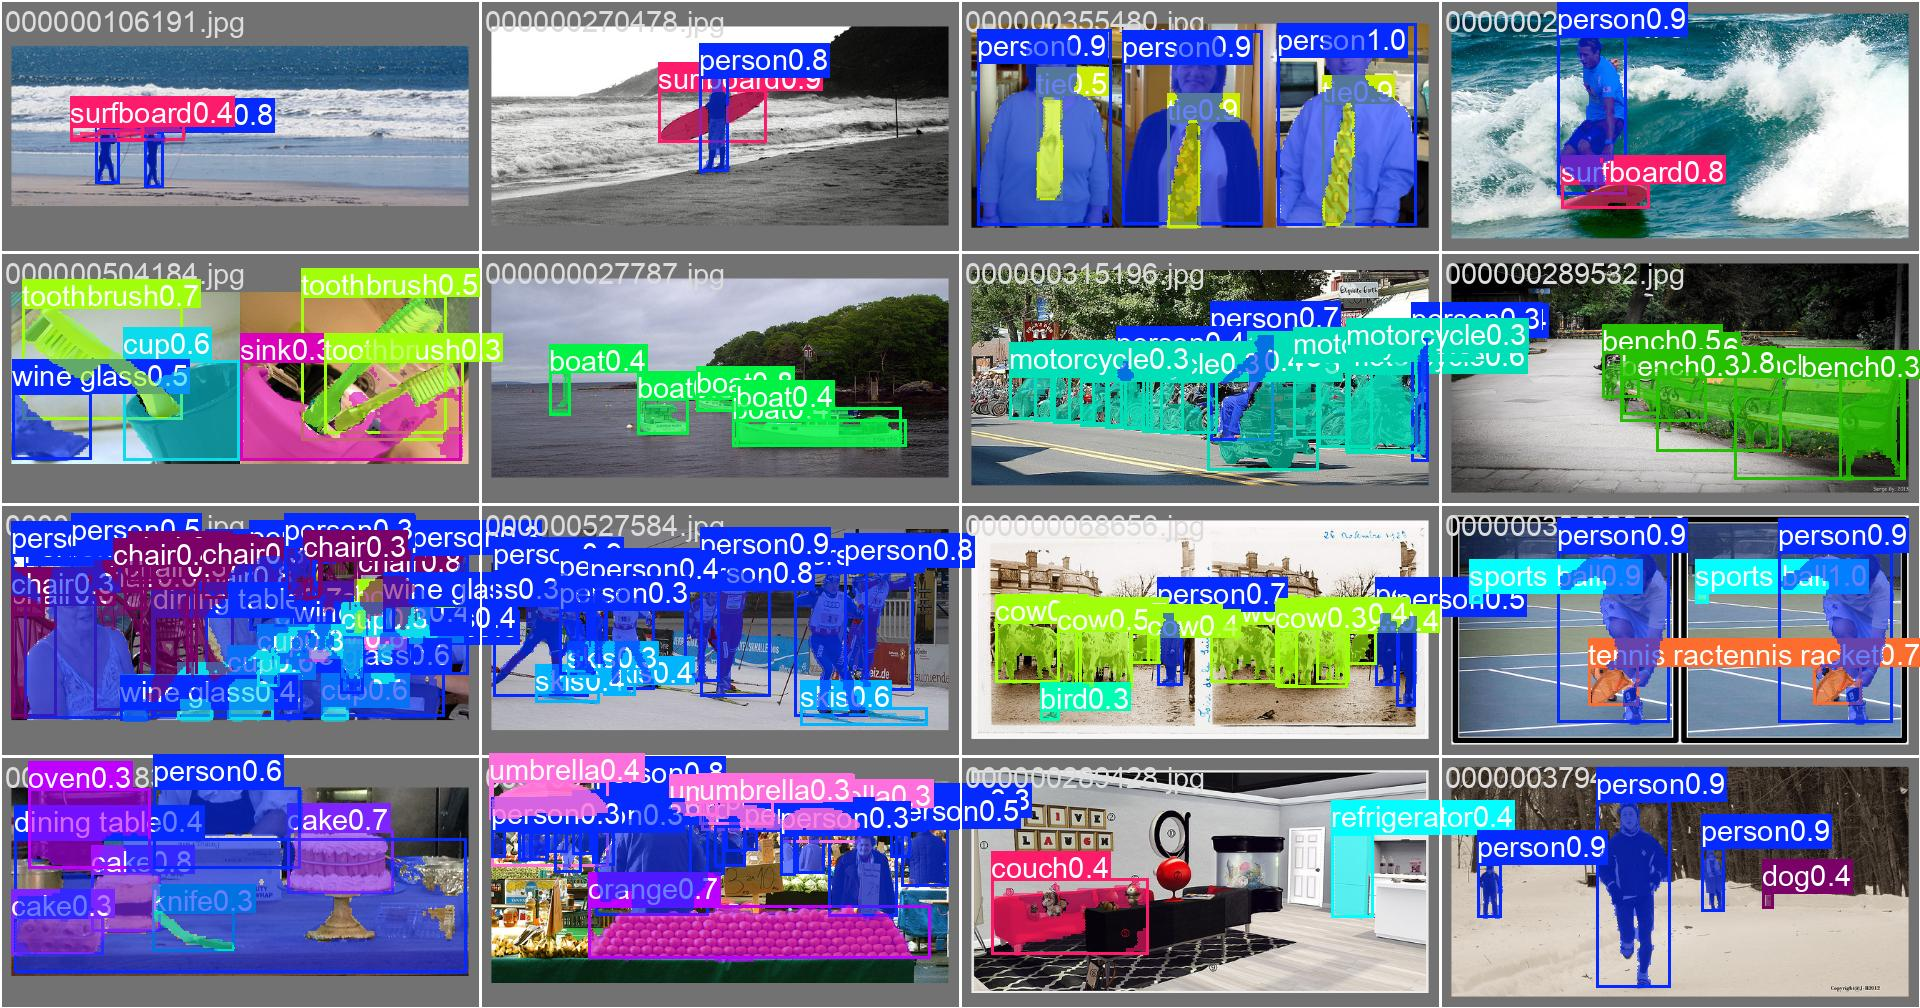
\includegraphics[width=\textwidth]{cualitativo_baseline.jpg}
    \end{column}
    \begin{column}{0.5\textwidth}
      \centering {\scriptsize Ajustado (8 clases)}\\
      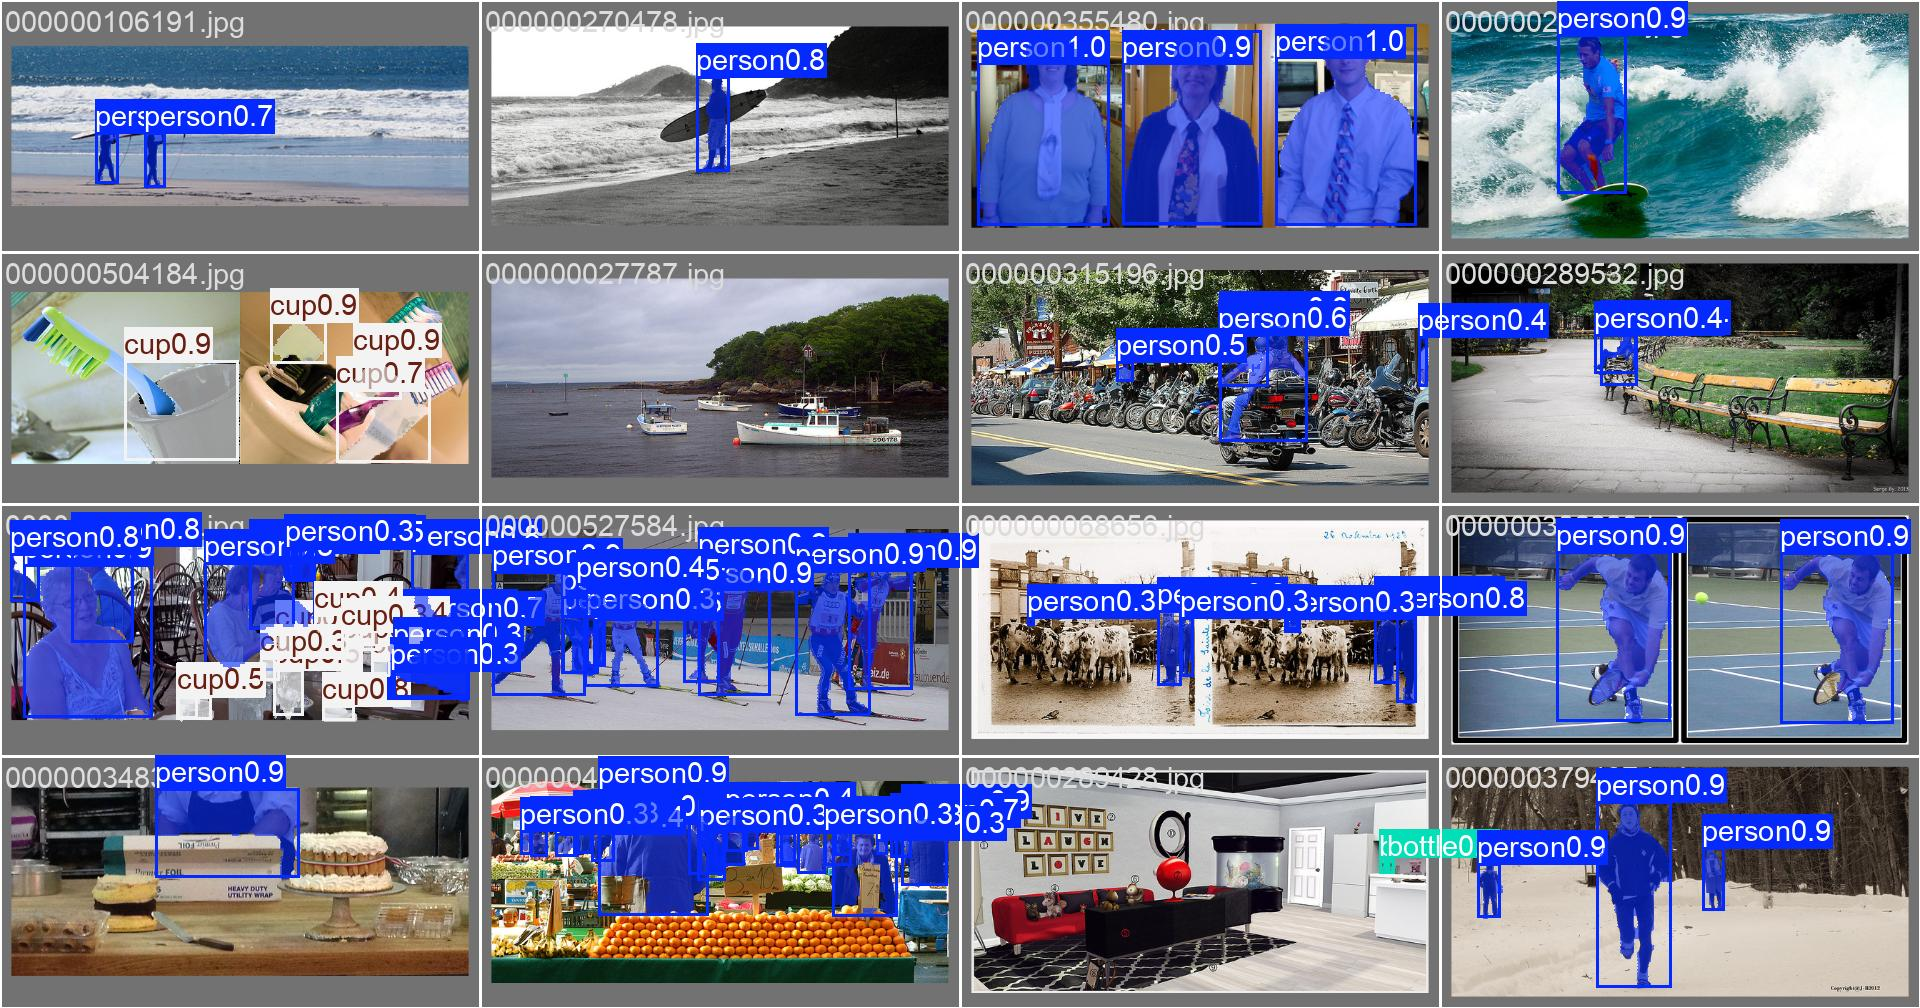
\includegraphics[width=\textwidth]{cualitativo_finetuned.jpg}
    \end{column}
  \end{columns}

  \vspace{0.3em}
  \begin{itemize}\footnotesize
    \item El baseline dispersa detecciones fuera de alcance
          (\texttt{refrigerator}, \texttt{surfboard}, \texttt{horse}, \texttt{umbrella},
          \texttt{pizza}, \texttt{cow}\ldots).
    \item El ajustado se concentra \textbf{exclusivamente} en las 8 clases: suprime por
          completo los falsos positivos de vocabulario. \emph{Esta} es su ventaja práctica,
          invisible para el mAP por clase.
  \end{itemize}
\end{frame}

% ============================================================================
\section{Sistema en tiempo real}

\begin{frame}{Tiempo real sobre CPU: el efecto de OpenVINO}
  \centering
  \small
  \begin{tabular}{@{}llcc@{}}
    \toprule
    \textbf{Plataforma} & \textbf{Formato} & \textbf{Latencia} & \textbf{FPS} \\
    \midrule
    Servidor, GPU RTX 5090 & PyTorch (\texttt{.pt}) & 5,1 ms/imagen & $\sim$198 \\
    PC personal, CPU Core Ultra 5 & PyTorch (\texttt{.pt}) & $\sim$59 ms/cuadro & 17 \\
    PC personal, CPU Core Ultra 5 & OpenVINO & $\sim$29 ms/cuadro & \textbf{35} \\
    \bottomrule
  \end{tabular}

  \vspace{0.4em}
  \begin{columns}[T]
    \begin{column}{0.33\textwidth}
      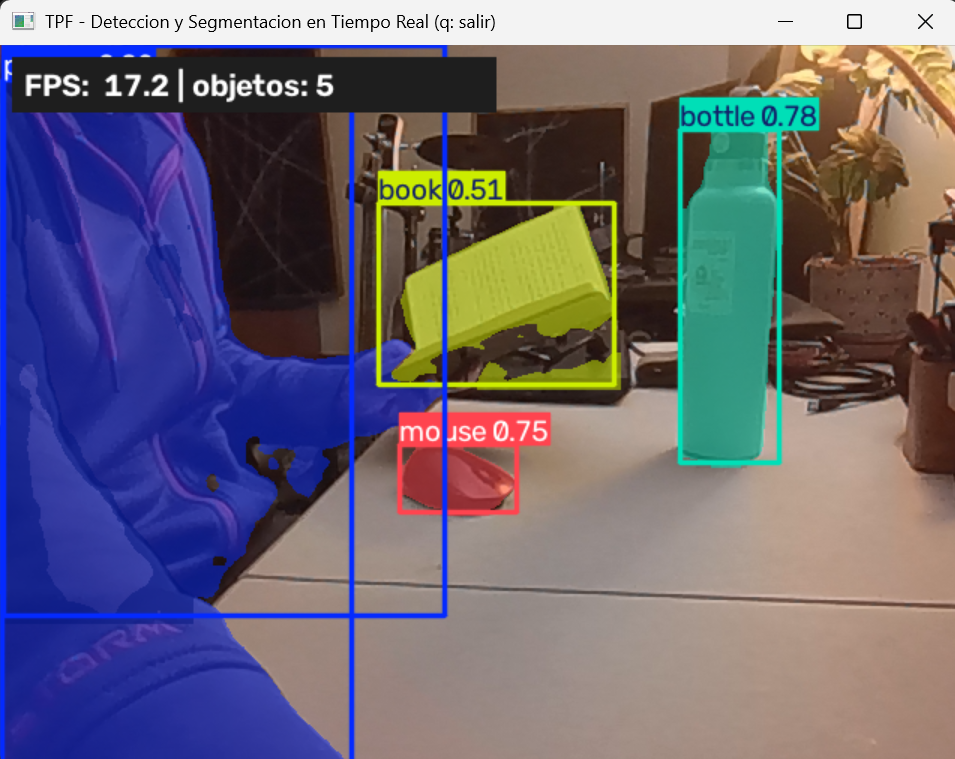
\includegraphics[width=\textwidth]{webcam_pt.png}\\
      \centering{\scriptsize PyTorch: 17,2 FPS}
    \end{column}
    \begin{column}{0.33\textwidth}
      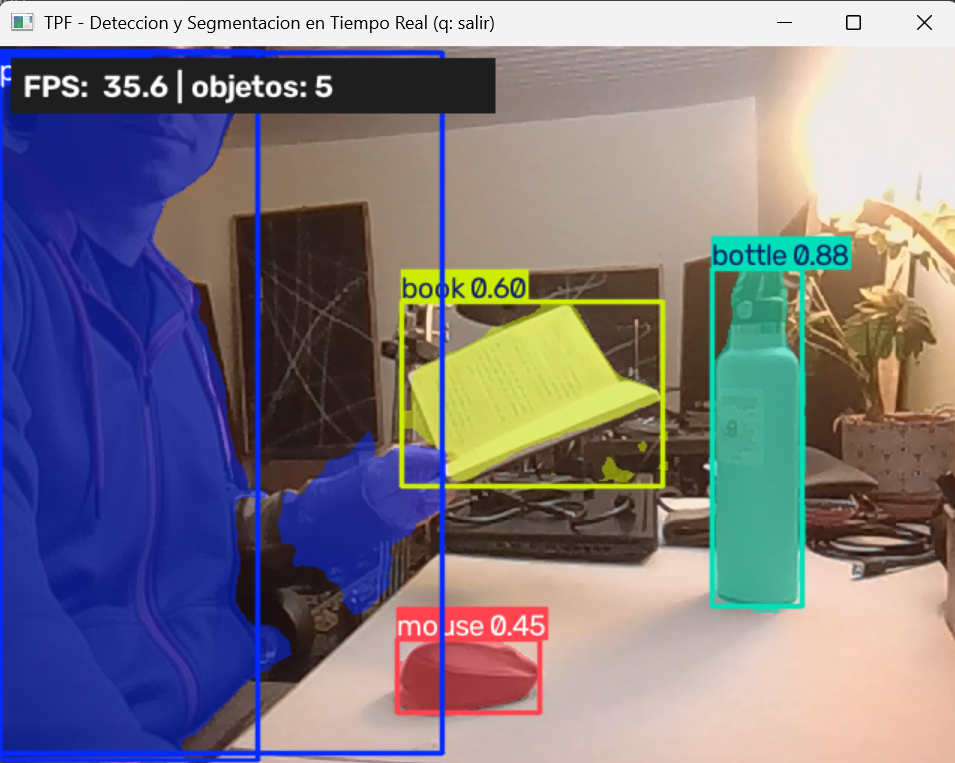
\includegraphics[width=\textwidth]{webcam_openvino.png}\\
      \centering{\scriptsize OpenVINO: 35,6 FPS}
    \end{column}
    \begin{column}{0.30\textwidth}
      \raggedright
      {\scriptsize \texttt{src/demo\_webcam.py}: captura con OpenCV, inferencia cuadro a
      cuadro y superposición de cajas, máscaras, etiquetas y FPS (media móvil
      exponencial).
      \vspace{0.4em}

      La PC de demostración \textbf{no tiene GPU con CUDA} $\Rightarrow$ se exporta el
      modelo a \textbf{OpenVINO}, la representación intermedia de Intel especializada
      para CPU.}
    \end{column}
  \end{columns}

  \vspace{0.2em}
  \centering{\scriptsize OpenVINO \textbf{duplica} la tasa de cuadros y supera el umbral de
  tiempo real (24--30 FPS) sin aceleración dedicada.}
\end{frame}

\begin{frame}{Despliegue en la nube: Hugging Face Spaces}
  \begin{columns}[T]
    \begin{column}{0.44\textwidth}
      La aplicación se desplegó en un \textbf{servidor público} con interfaz Gradio: quien
      la evalúe solo abre un enlace, sin descargar ni instalar nada.
      \vspace{0.6em}

      \textbf{Dos modos de uso}
      \begin{itemize}\footnotesize
        \item \textbf{Imagen} --- sube una fotografía; devuelve cajas, máscaras y recuento
              de objetos por clase.
        \item \textbf{Webcam en vivo} --- inferencia cuadro a cuadro sobre la cámara del
              navegador, con umbral de confianza y resolución expuestos.
      \end{itemize}
      \vspace{0.5em}
      {\scriptsize Los pesos viajan dentro del repositorio del Space: el modelo se ejecuta
      íntegramente en la nube.}
    \end{column}
    \begin{column}{0.52\textwidth}
      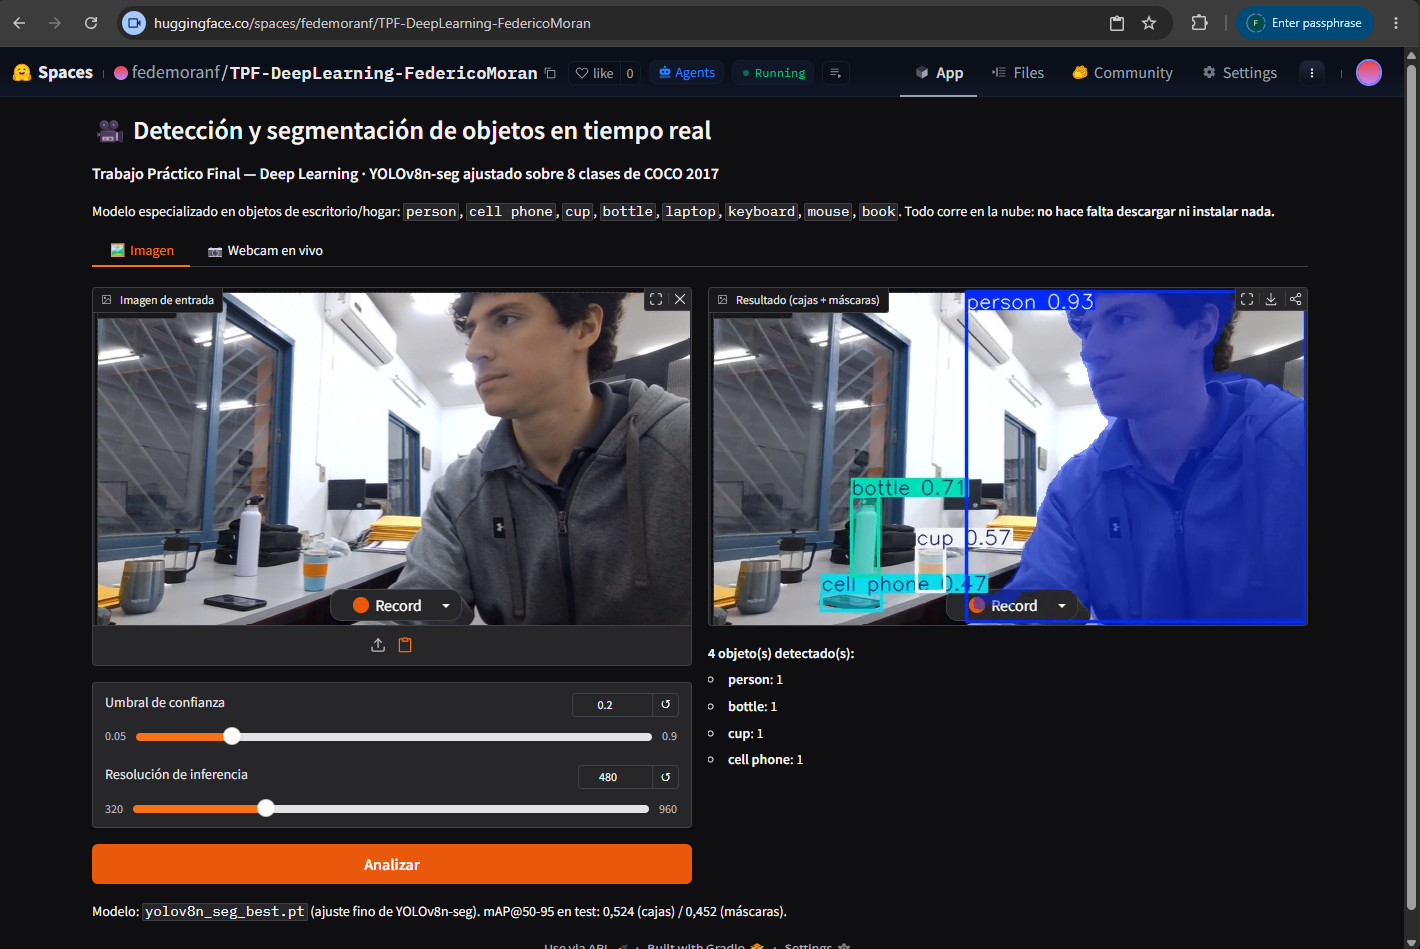
\includegraphics[width=\textwidth]{prueba_huggingface.png}
    \end{column}
  \end{columns}
\end{frame}

\begin{frame}[plain]
  \centering
  \vfill
  {\Huge\bfseries\color{azul} Demostración en vivo}
  \vfill
  {\large Detección y segmentación de instancias sobre cámara web}\\[0.5em]
  {\normalsize CPU Intel Core Ultra 5 226V --- sin GPU dedicada}
  \vfill
\end{frame}

% ============================================================================
\section{Conclusiones}

\begin{frame}{Conclusiones}
  \begin{enumerate}
    \item \textbf{La evaluación rigurosa es tan determinante como el modelo.} Se
          corrigieron dos sesgos optimistas: la fuga en el propio \emph{split} y el
          preentrenamiento del baseline sobre el mismo pozo de datos del que salió nuestro
          test. Bajo una comparación imparcial en val2017 el modelo ajustado es
          \textbf{competitivo} con el preentrenado.
    \vspace{0.3em}
    \item \textbf{Con un vocabulario que es subconjunto del preentrenamiento, el aporte del
          ajuste fino es la especialización, no el mAP:} elimina las detecciones espurias
          de las 72 categorías fuera de alcance.
    \vspace{0.3em}
    \item \textbf{El error dominante es la omisión, no la confusión entre clases:} el
          desempeño por clase lo gobiernan las características visuales y la calidad de
          anotación de cada categoría.
    \vspace{0.3em}
    \item \textbf{La segmentación de instancias en tiempo real es viable sobre una CPU de
          consumo:} 35~FPS sostenidos con OpenVINO, el doble que el formato PyTorch
          original.
    \vspace{0.3em}
    \item \textbf{El pipeline es reproducible de extremo a extremo}, con semillas fijas y
          controles de integridad sobre los archivos exportados.
  \end{enumerate}
\end{frame}

\begin{frame}{Limitaciones y trabajo futuro}
  \begin{columns}[T]
    \begin{column}{0.48\textwidth}
      \textbf{Limitaciones}
      \begin{itemize}\footnotesize
        \item \textbf{Desbalance de clases:} \texttt{person} concentra el 74,2\,\% de las
              instancias; \texttt{mouse} y \texttt{keyboard} tienen menos de 150 ejemplos
              de entrenamiento. No se corrigió artificialmente: es la estadística del
              dominio de despliegue.
        \item \textbf{Calidad de la anotación de referencia:} \texttt{book} tiene límites
              ambiguos en COCO, lo que impone un techo a su desempeño medible.
        \item \textbf{Escala del conjunto:} 3.000 imágenes son dos órdenes de magnitud
              menos que el preentrenamiento; por eso congelar el backbone es determinante.
      \end{itemize}
    \end{column}
    \begin{column}{0.48\textwidth}
      \textbf{Trabajo futuro}
      \begin{itemize}\footnotesize
        \item \textbf{Ampliar el conjunto de datos}, en especial las clases raras.
        \item \textbf{Atacar el recall} de instancias pequeñas: inferencia en mosaico
              (\emph{tiling}) o mayor resolución de entrada.
        \item \textbf{Variantes de mayor capacidad} (YOLOv8s-seg), midiendo el intercambio
              precisión--latencia sobre la CPU de despliegue.
        \item \textbf{Cuantización INT8} con OpenVINO para elevar aún más los FPS.
        \item[$\Rightarrow$] La única vía para \textbf{superar} genuinamente al baseline es
              entrenar con datos del \textbf{dominio real} (imágenes de webcam), no con
              más COCO.
      \end{itemize}
    \end{column}
  \end{columns}
  \vspace{0.3em}
  \centering
  {\Large\color{azul}\bfseries ¿Preguntas?}
\end{frame}

% ============================================================================
\appendix

\begin{frame}[plain]
  \centering
  \vfill
  {\Large\bfseries\color{gris} Diapositivas de respaldo}
  \vfill
\end{frame}

\begin{frame}{Respaldo --- Curvas de aprendizaje}
  \centering
  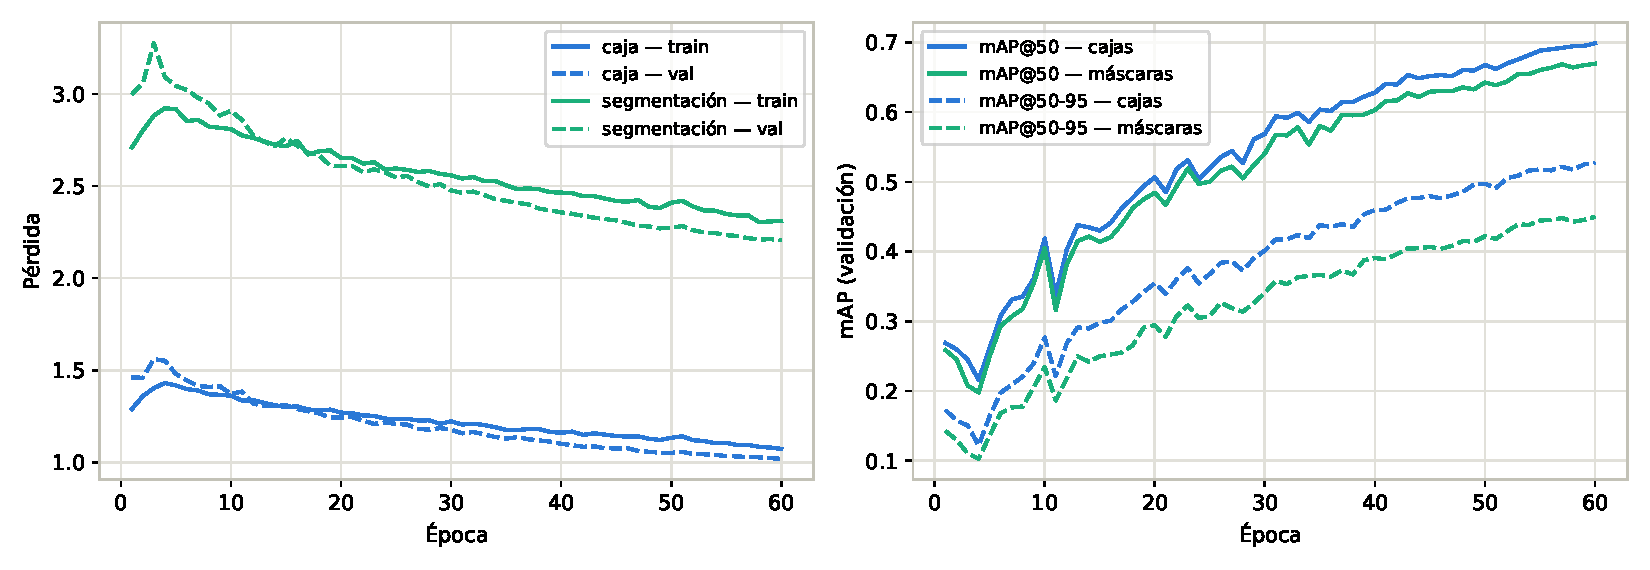
\includegraphics[width=0.88\textwidth]{curvas_entrenamiento.pdf}

  \vspace{0.3em}
  \begin{itemize}\footnotesize
    \item Las pérdidas de caja y segmentación decrecen de forma sostenida, sin divergencia:
          no hay sobreajuste.
    \item El mAP de validación crece rápido y se estabiliza en una meseta (mAP@50-95 de
          máscaras hasta 0,283), coherente con un modelo de \emph{backbone} congelado.
    \item La pérdida de validación se ubica \textbf{por encima} de la de entrenamiento,
          como corresponde a la brecha de generalización sobre una partición reservada.
  \end{itemize}
\end{frame}

\begin{frame}{Respaldo --- Cuánto valía la ventaja de fuga del baseline}
  \begin{alertblock}{La comparación que \emph{no} se presentó, y por qué}
    \footnotesize
    Evaluar al preentrenado sobre \emph{nuestra} partición de prueba (muestreada de COCO
    train2017, con la que él fue entrenado) lo favorece: mide, en parte, su memoria sobre
    sus propios datos de entrenamiento. Por eso la comparación del cuerpo de la
    presentación se hace únicamente sobre COCO val2017.
  \end{alertblock}

  \vspace{0.4em}
  \centering
  \small
  \begin{tabular}{@{}lcccc@{}}
    \toprule
    & \multicolumn{2}{c}{\textbf{Preentrenado}} & \multicolumn{2}{c}{\textbf{Ajustado}} \\
    \cmidrule(lr){2-3}\cmidrule(lr){4-5}
    mAP@50-95 & Cajas & Máscaras & Cajas & Máscaras \\
    \midrule
    Nuestro test (de train2017) --- \emph{sesgado} & 0,403 & 0,342 & 0,292 & 0,246 \\
    \textbf{COCO val2017 --- imparcial} & \textbf{0,329} & \textbf{0,277} & \textbf{0,275} & \textbf{0,236} \\
    \bottomrule
  \end{tabular}

  \vspace{0.6em}
  \begin{exampleblock}{La magnitud del sesgo}
    \footnotesize
    Al pasar a datos no vistos el baseline \textbf{cae} de 0,342 a 0,277 en máscaras,
    mientras que el ajustado apenas varía (0,246 $\to$ 0,236): para él ambas particiones son
    igualmente novedosas. Cerca de \textbf{dos tercios de la brecha aparente} eran la
    ventaja de fuga del baseline, no un defecto del modelo ajustado.
  \end{exampleblock}
\end{frame}

\begin{frame}{Respaldo --- Control de la fuga de datos}
  \begin{alertblock}{Un riesgo real, detectado y corregido}
    \footnotesize
    FiftyOne etiqueta cada muestra descargada con su \emph{split de origen}
    (\texttt{train}, por venir de COCO train2017). Esa etiqueta \textbf{colisiona} con la
    de la partición propia: \texttt{match\_tags('train')} devuelve las 5.000 imágenes, no
    las 3.000 previstas, y el modelo entrena sobre validación y prueba.
  \end{alertblock}

  \vspace{0.4em}
  \begin{block}{Tres correcciones encadenadas}
    \footnotesize
    \begin{enumerate}
      \item \texttt{untag\_samples} elimina las etiquetas de split de origen \emph{antes}
            de particionar.
      \item \texttt{rmtree} del directorio de destino antes de exportar: el exportador de
            FiftyOne \textbf{fusiona} por defecto con lo que ya haya en disco.
      \item Un \texttt{assert} sobre los \textbf{archivos exportados} verifica que las
            particiones sean disjuntas y midan 3.000 / 750 / 1.250.
    \end{enumerate}
  \end{block}

  \vspace{0.3em}
  \begin{exampleblock}{Verificación sobre los archivos, no sobre las etiquetas}
    \footnotesize
    El control definitivo se hace sobre lo que el entrenador \emph{realmente lee del disco}.
    Síntoma que delató el problema: el log de Ultralytics decía
    \texttt{train: Scanning\ldots 5000 images}.
  \end{exampleblock}
\end{frame}

\begin{frame}{Respaldo --- Protocolo de evaluación}
  \begin{columns}[T]
    \begin{column}{0.46\textwidth}
      \textbf{IoU} --- solapamiento entre la predicción $P$ y la anotación $G$:
      \begin{equation*}
        IoU(P,G) = \frac{|P \cap G|}{|P \cup G|}
      \end{equation*}
      Se aplica \textbf{tanto a cajas como a máscaras}. Una predicción es verdadero
      positivo si su IoU con una anotación de la misma clase supera un umbral.
      \vspace{0.6em}

      \textbf{AP} --- área bajo la curva precisión--recall de una clase.\\
      \textbf{mAP} --- promedio de las AP sobre las clases.
    \end{column}
    \begin{column}{0.5\textwidth}
      \begin{block}{Las dos variantes estándar}
        \footnotesize
        \textbf{mAP@50} --- umbral de IoU de 0,5. Criterio laxo: mide si el objeto fue
        encontrado.
        \vspace{0.4em}

        \textbf{mAP@50-95} --- promedio sobre umbrales de 0,5 a 0,95 en pasos de 0,05.
        Criterio estricto: premia la \textbf{precisión de la localización}. Es la métrica
        principal de este trabajo.
      \end{block}
      \vspace{0.4em}
      {\footnotesize Todo se calcula por separado para \textbf{cajas} (detección) y
      \textbf{máscaras} (segmentación), sobre la partición de prueba
      (1.250 imágenes, 7.117 instancias), reservada de principio a fin.}
    \end{column}
  \end{columns}
\end{frame}

\begin{frame}{Respaldo --- Configuración completa del entrenamiento}
  \centering
  \small
  \begin{tabular}{@{}ll@{}}
    \toprule
    \textbf{Parámetro} & \textbf{Valor} \\
    \midrule
    Modelo base & \texttt{yolov8n-seg.pt} (preentrenado en COCO) \\
    Capas congeladas & \texttt{freeze=10} (backbone); se entrenan neck y cabeza \\
    Épocas & 150 (early stopping, paciencia 50) \\
    Resolución de entrada & $640\times640$ (letterbox) \\
    Tamaño de lote & 32 \\
    Procesos de precarga & 4 \\
    Optimizador & AdamW (selección automática), $lr_0 = 8{,}33\times10^{-4}$, momento 0,9 \\
    Decaimiento de pesos & $5\times10^{-4}$ \\
    Precisión mixta (AMP) & Sí \\
    Semilla & 42 (modo determinista) \\
    Hardware & GPU NVIDIA RTX 5090 (32~GB) \\
    Duración & 132 minutos (se detuvo en la época 140) \\
    \bottomrule
  \end{tabular}

  \vspace{0.8em}
  {\footnotesize El lote y los procesos de precarga se fijaron explícitamente para acotar
  el consumo de memoria en un servidor compartido. El punto de control se selecciona por
  la \textbf{métrica de aptitud sobre validación}.}
\end{frame}

\begin{frame}{Respaldo --- Preguntas anticipadas (I)}
  \small
  \textbf{¿Por qué YOLOv8 y no una arquitectura de dos etapas (Mask R-CNN)?}\\
  El requisito de tiempo real sobre CPU descarta las arquitecturas de dos etapas. YOLOv8-seg
  resuelve detección y segmentación en una sola pasada, con costo de máscara casi constante
  gracias a los prototipos.
  \vspace{0.6em}

  \textbf{¿Por qué la variante nano y no small o medium?}\\
  Es la única que sostiene tiempo real sobre la CPU de despliegue. La variante \emph{small}
  quedó identificada como trabajo futuro, con la latencia como criterio de decisión.
  \vspace{0.6em}

  \textbf{¿Por qué AdamW y esa tasa de aprendizaje?}\\
  Selección automática de Ultralytics (\texttt{optimizer='auto'}), que fija
  $lr_0 = 8{,}33\times10^{-4}$ y momento 0,9 en función del tamaño del conjunto y del lote.
  \vspace{0.6em}

  \textbf{¿Por qué no se corrigió el desbalance con pesos de clase o focal loss?}\\
  El desbalance es la estadística natural del dominio y se traslada al escenario de
  despliegue. Corregirlo artificialmente optimizaría una distribución que no es la de uso.
\end{frame}

\begin{frame}{Respaldo --- Preguntas anticipadas (II)}
  \small
  \textbf{¿Cómo se garantiza que no hay fuga de datos entre train y test?}\\
  Con dos controles independientes: (i)~\texttt{untag\_samples} elimina las etiquetas de
  split de origen de FiftyOne antes de particionar; (ii)~un \texttt{assert} verifica, sobre
  los \emph{archivos exportados} —que es lo que el entrenador realmente lee—, que las tres
  particiones sean disjuntas y midan 3.000 / 750 / 1.250.
  \vspace{0.6em}

  \textbf{¿Por qué la pérdida de validación estuvo por debajo de la de entrenamiento en
  corridas previas?}\\
  Era un síntoma. Con particiones correctas la pérdida de validación queda \emph{por
  encima}, como corresponde. En una corrida anterior, val estaba contenida en train.
  \vspace{0.6em}

  \textbf{¿El aumento de datos se aplica también a las máscaras?}\\
  Sí. Ultralytics transforma imágenes y polígonos de forma consistente; \emph{mosaic}
  recompone las cuatro máscaras en el lienzo combinado.
  \vspace{0.6em}

  \textbf{¿Por qué \texttt{close\_mosaic}?}\\
  \emph{Mosaic} produce imágenes de estadística artificial; \texttt{close\_mosaic=10} lo
  desactiva en las últimas 10 épocas para afinar sobre imágenes naturales. En esta corrida
  el \emph{early stopping} (época 140) se adelantó a esa fase, sin perjuicio para la
  convergencia.
\end{frame}

\begin{frame}{Respaldo --- Preguntas anticipadas (III)}
  \small
  \textbf{¿Por qué el baseline se evalúa con 80 clases y el modelo ajustado con 8?}\\
  Porque son los vocabularios nativos de cada modelo; de las AP del baseline se extraen las
  8 clases de interés sobre las mismas imágenes. Y ---clave--- la comparación principal se
  hace sobre COCO \textbf{val2017}, no sobre nuestra partición de train2017: el preentrenado
  fue entrenado sobre train2017, así que evaluarlo ahí lo favorece. Sobre val2017, no vista
  por ninguno de los dos, la comparación es limpia.
  \vspace{0.6em}

  \textbf{¿La partición de prueba se usó alguna vez para tomar decisiones?}\\
  No. El punto de control se selecciona por el mAP@50-95 de máscaras sobre
  \textbf{validación}. La prueba se evalúa una sola vez, al final.
  \vspace{0.6em}

  \textbf{¿Los FPS dependen del modelo entrenado?}\\
  No. La latencia depende de la arquitectura y del formato de ejecución, no de los valores
  de los pesos. Las mediciones de 17 y 35 FPS son estables entre corridas.
  \vspace{0.6em}

  \textbf{¿Qué pasa si la cámara falla en la demo?}\\
  Hay un video de respaldo: \texttt{python src/demo\_webcam.py --source respaldo.mp4}.
\end{frame}

\begin{frame}{Respaldo --- Correspondencia con la consigna}
  \centering
  \small
  \begin{tabular}{@{}ll@{}}
    \toprule
    \textbf{Requisito} & \textbf{Dónde se cumple} \\
    \midrule
    Detección y/o segmentación & YOLOv8n-seg ajustado: cajas + máscaras \\
    Preprocesamiento y \emph{data augmentation} & Notebooks 01 y 02 \\
    Métricas estándar (mAP, IoU) & Notebook 03: mAP@50 y mAP@50-95 \\
    Inferencia en tiempo real & \texttt{src/demo\_webcam.py} (FPS en pantalla) \\
    Pipeline completo & Notebooks 01$\rightarrow$03 + \texttt{src/} \\
    Modelo entrenado & \texttt{models/yolov8n\_seg\_best.pt} \\
    Reporte técnico con código por paso & \texttt{reporte/informe.pdf} \\
    Demo en la nube, solo un enlace & Hugging Face Space (Gradio) \\
    Presentación oral con demo & Este documento + demo en vivo \\
    \bottomrule
  \end{tabular}
\end{frame}

\end{document}
